
\subsection{Suppression de la publicité}
Nous avons remarqué que l'application possède une seule point d'entrée pour afficher la publicité.
L'application charge la vue pour la publicité dans la méthode onCreate().
\begin{figure}[hp]
	      \begin{center}
		\fbox{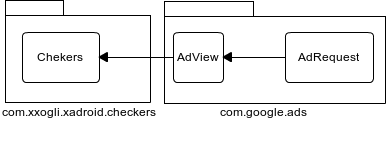
\includegraphics[scale=0.7]{pub}}
	      \end{center}
	\legend{Affichage de la publicité}
\end{figure}

\begin{table}[here]
    \begin{center}
	\begin{tabular}{|l|}
	\hline
	const/16 v1, 0x50 \\[0.2cm]
	
	invoke-virtual {v0, v1}, Lcom/google/ads/AdView;->setGravity(I)V \\[0.2cm]

	new-instance v1, Lcom/google/ads/AdRequest; \\[0.2cm]

	invoke-direct/range {v1 .. v1}, Lcom/google/ads/AdRequest;-><init>()V \\[0.2cm]

	invoke-virtual {v0, v1}, Lcom/google/ads/AdView;->loadAd(Lcom/google/ads/AdRequest;)V \\
	\hline
	\end{tabular}
    \end{center}
    \caption{\label{}code smali pour la publicité}
\end{table} 
La variable v1 contient l'instance de la classe \textit{com.google.ads.AdRequest} qui est le point d'entrée de la publicité dans l'application.
La variable v0 est la vue \textit{com.google.ads.AdView} associée à la publicité. Le chargement de la publicité se fait par la méthode \textit{loadAd(AdRequest adrequest)}.
